\section{Proceso B\'asico del Reconocimiento del Habla}

\begin{frame}{Proceso B\'asico del Reconocimiento del Habla}

\begin{quote}
\emph{La b\'usqueda de la oraci\'on m\'as probable perteneciente al lenguaje L, dada la entrada ac\'ustica X.}
\end{quote}

\begin{align}
\hat{W} = \argmax_{W \in L} \overbrace{P(O|W)}^\text{M. ac\'ustico}\overbrace{P(W)}^\text{M. de lenguaje}
\label{eq:asrFundamental}
\end{align}
\end{frame}

\begin{frame}{Proceso B\'asico del Reconocimiento del Habla (2)}

\begin{figure}[H] 
\centering
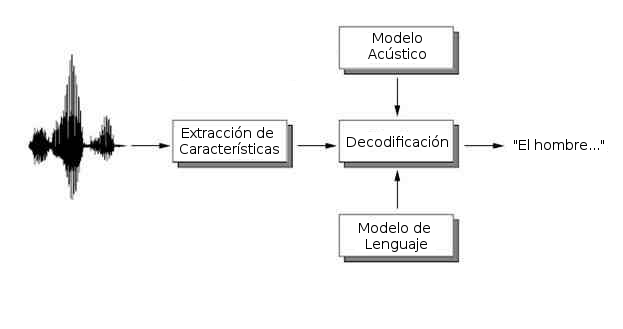
\includegraphics[width=0.8\textwidth]{./graphics/proceso.png}
\caption{Proceso del reconocimiento del habla. Traducido a partir de \protect\cite{VerenichASR}.}
\label{figure:proceso}
\end{figure}
\end{frame}

\begin{frame}{Proceso B\'asico del Reconocimiento del Habla (3)}
\framesubtitle{Fase 1: Extracci\'on de caracter{\'\i}sticas}
\begin{figure}[H]
\centering
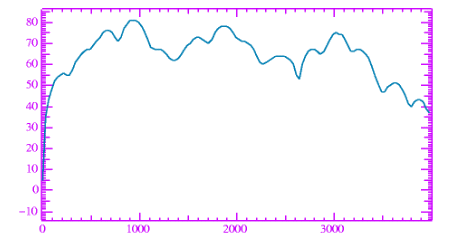
\includegraphics[width=0.4\linewidth]{./graphics/formants.png}
\caption{Representaci\'on del espectro en el cual pueden identificarse los picos espectrales o formantes 
\cite{Jurafsky}.}
\label{figure:formants}
\end{figure}


\begin{figure}[H]
\centering
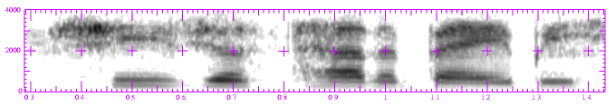
\includegraphics[width=0.7\linewidth]{./graphics/spectrogram.png}
\caption{Representaci\'on de un espectrograma, puede verse como una colecci\'on de espectros como la 
    figura~\ref{figure:formants} ubicados uno despu\'es otro \cite{Jurafsky}.}
\label{figure:spectrogram}
\end{figure}

\end{frame}

\begin{frame}{Proceso B\'asico del Reconocimiento del Habla (4)}
\framesubtitle{Fase 1: Extracci\'on de caracter{\'\i}sticas}

\begin{figure}[H] 
\centering
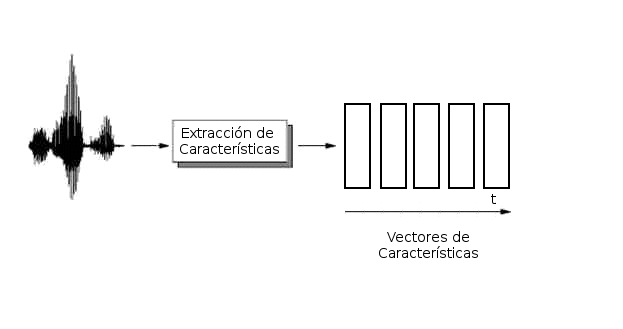
\includegraphics[width=0.8\textwidth]{./graphics/extraccion.png}
\caption{Fase de extracci\'on de caracter{\'\i}sticas. Gr\'afico basado en \cite{VerenichASR}.}
\label{figure:hmm}
\end{figure}
\end{frame}


\begin{frame}{Proceso B\'asico del Reconocimiento del Habla (5)}
\framesubtitle{Fase 2: Decodificaci\'on: Modelo de Lenguaje}
Sean:
\begin{itemize}
    \item $V$, el conjunto finito de palabras que componen un lenguaje, tambi\'en conocido como vocabulario.
    \item $V^\dag$, el conjunto infinito de oraciones que pueden formarse con palabras pertenecientes 
        al vocabulario.
    \item $x_1,x_2,\ldots,x_n$, una secuencia de palabras de longitud $n$.
\end{itemize}

Un modelo de lenguaje \cite{CollinsLanguage} consiste en un conjunto finito $V$ y una funci\'on 
de probabilidad $P(x_1,x_2,\ldots,x_n)$ tal que:
\begin{enumerate}

\item $\forall (x_1,x_2,\ldots,x_n) \in V^\dag, P(x_1,x_2,\ldots,x_n) \ge 0$

\item $\displaystyle \sum_{(x_1,x_2,\ldots,x_n) \in V^\dag} P(x_1,x_2,\ldots,x_n) = 1$
\end{enumerate}
\end{frame}

\begin{frame}{Proceso B\'asico del Reconocimiento del Habla (6)}
\framesubtitle{Fase 2: Decodificaci\'on - Modelo Acústico}

\begin{itemize}
    \item Modelos Ocultos de Markov
    \item Diccionario Fonético
\end{itemize}

\begin{figure}[H] 
\centering
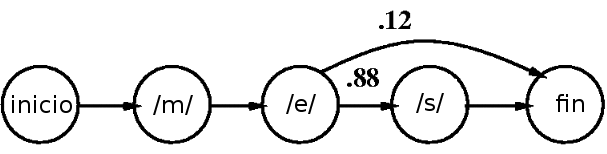
\includegraphics[width=0.5\textwidth]{./graphics/hmm_palabra.png}
\caption{Representaci\'on ac\'ustica de la palabra ``mes''. Basado en \cite{Jurafsky}.}
\label{figure:hmm-palabra}
\end{figure}

\end{frame}

\begin{frame}{Proceso B\'asico del Reconocimiento del Habla (7)}
\framesubtitle{Fase 2: Decodificaci\'on - Búsqueda}

\begin{itemize}
    \item Algoritmo de Viterbi.
    \item Algoritmo A*.
\end{itemize}

\begin{figure}[H] 
\centering
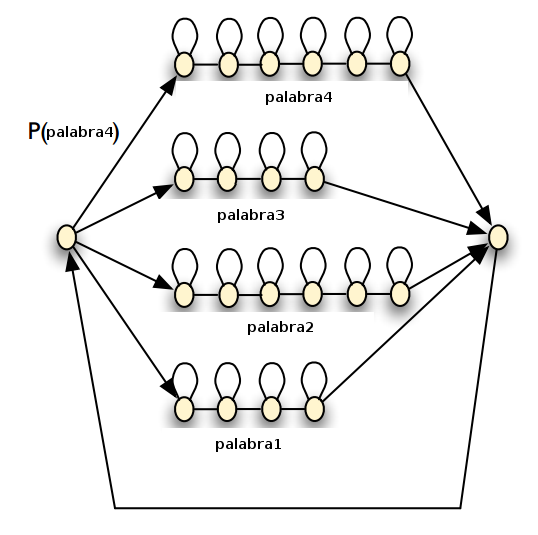
\includegraphics[width=0.5\textwidth]{./graphics/espacio.png}
\caption{Espacio de b\'usqueda para un lenguaje simple de cuatro palabras. Traducido a partir de \cite{RenalsSearch}.}
\label{figure:espacio-busqueda}
\end{figure}

\end{frame}


\begin{frame}{Proceso B\'asico del Reconocimiento del Habla (8)}
\framesubtitle{Fase 2: Decodificaci\'on}
\begin{figure}[H] 
\centering
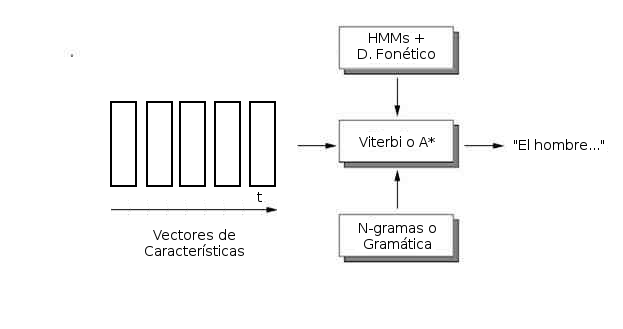
\includegraphics[width=0.8\textwidth]{./graphics/decodificacion.png}
\caption{Fase de decodificaci\'on. Gr\'afico basado en \cite{VerenichASR}.}
\label{figure:decoding}
\end{figure}
\end{frame}
